\section{Experimental results}

    We evaluated the proposed approach on a dataset consisting of $N = 4$ books in $I = 4$ poses. We used two pairs of books which are ambiguous from the back and unambigious from the front. \figref{fig:object_dataset} shows the covers of all the books used for the experiment. Each book was trained in $I = 4$ discrete poses: up and down with the spine visible and not visible. This leads to $4$ actions: stay, rotate, flip, and flip-rotate. All poses are presented in \figref{fig:pose_dataset}. 
    
    \begin{figure}[h]
        
\includegraphics[width = 0.2\columnwidth]{pics/math_cover1_ok.jpg}
        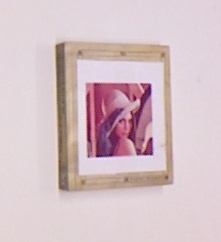
\includegraphics[width = 0.2\columnwidth]{pics/math_cover2_ok.jpg}
        
\includegraphics[width = 0.2\columnwidth]{pics/first_cover1.jpg}
        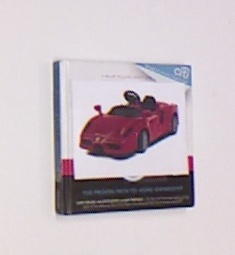
\includegraphics[width = 0.2\columnwidth]{pics/first_cover2.jpg}
        \caption{All four books with the oriented with the cover up and the spine visible.}
        \label{fig:object_dataset} % TODO: spine is not visible in one of these! 
    \end{figure}

    \begin{figure}[h]
        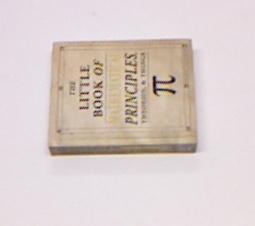
\includegraphics[width = 0.2\columnwidth]{pics/math_cover1.jpg}
        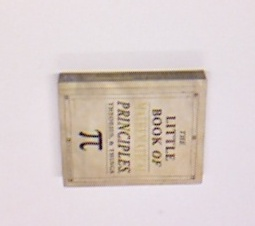
\includegraphics[width = 0.2\columnwidth]{pics/math_cover1_rot.jpg}
        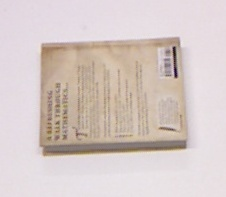
\includegraphics[width = 0.2\columnwidth]{pics/math_down.jpg}
        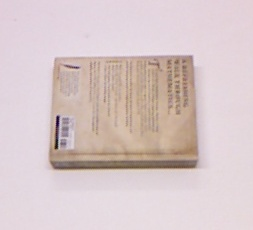
\includegraphics[width = 0.2\columnwidth]{pics/math_down_rot.jpg}
        \caption{All poses of a single book. From left to right: up, up-spine, down, down-spine} % TODO: spine and no spine are messed up
    \label{fig:pose_dataset}
    \end{figure}

    $M = 654$ unique features were extracted from a set of ideal images of each object-pose pair. We recorded $R = 100$ training sample for each object-pose pair to learn the likelihood distribution $\prob{f|o,p}$. For the ambiguous case, we use the same training images due to an overfitting issue in our object recognition algorithm. Our experimental setup consists of a Microsoft Kinect sensor which we use as a RGB camera. All the actions are executed by a human and we assume that actions are nearly perfect. 

    \subsection{Object recognition}
        In order to evaluate the object recognition model, we trained the model on $80$ samples and held out $20$ samples for cross validation. The average prediction accuracy results for the unambiguous cases are presented in \tabref{tab:accuracy}. It is worth emphasizing that we did not include the ambiguous poses in the cross validation results because these ambiguous cases were designed to cause static object recognition to fail. Note that all classification errors were due to confusion about whether the spine was visible or not.
        
        \begin{table}[h]
                \centering
                \begin{tabular}{|c|c|}
                \hline
                Average Training Accuracy & Average Cross Validation Accuracy \\
                \hline
                99.67\% & 93.75\% \\
                \hline
                \end{tabular}
                \caption{Average classification accuracy for static object recognition of objects in unambiguous poses.}
                \label{tab:accuracy}
        \end{table}

    \subsection{Action selection}

        Our action selection experiment is represented by the decision tree in \figref{fig:tree}.

        \begin{figure}[h]
            \centering
            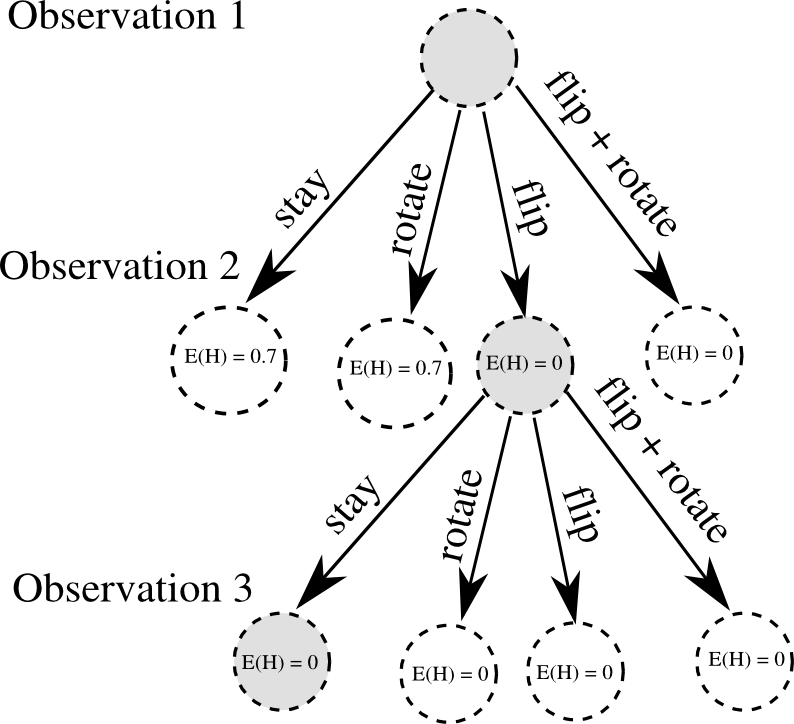
\includegraphics[scale=0.7]{pics/tree_small.png}
            \caption{Decision tree for the action selection experiment. Each node represents the expected entropy of the posterior for a given action. Colored nodes indicate the optimal action. Right: observed images.}
            \label{fig:tree} % TODO: Fix the images -- this is neither spine or not spine! Separate the tree from the observations and we'll have them in separate figures. Also fix the resolution
        \end{figure}

        First, the ambiguous back of the book pose is observed as shown in \figref{fig:expObs} (left). As expected, the posterior probabilities is split between the two ambiguous books shown in \figref{fig:expObsPost} (left).

        \begin{figure}[h]
            \centering
            \begin{tabular}{cc} 
                
\includegraphics[scale=0.05]{pics/obs1.jpg}
                    &
                
\includegraphics[scale=0.05]{pics/obs2.jpg}
            \end{tabular}
            \caption{Left: the first ambigious observation. Right: the second unambiguous observation.}
            \label{fig:expObs}
        \end{figure}

        \begin{figure}[h]
            \centering
            \begin{tabular}{cc} 
                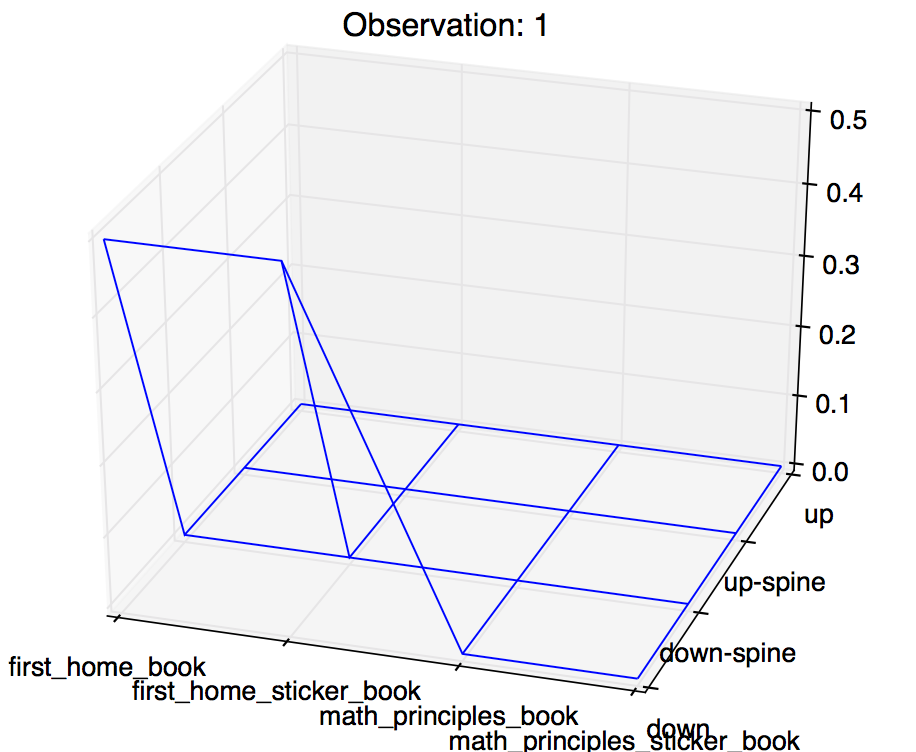
\includegraphics[scale=0.4]{pics/experimentObs1.png}
                    &
                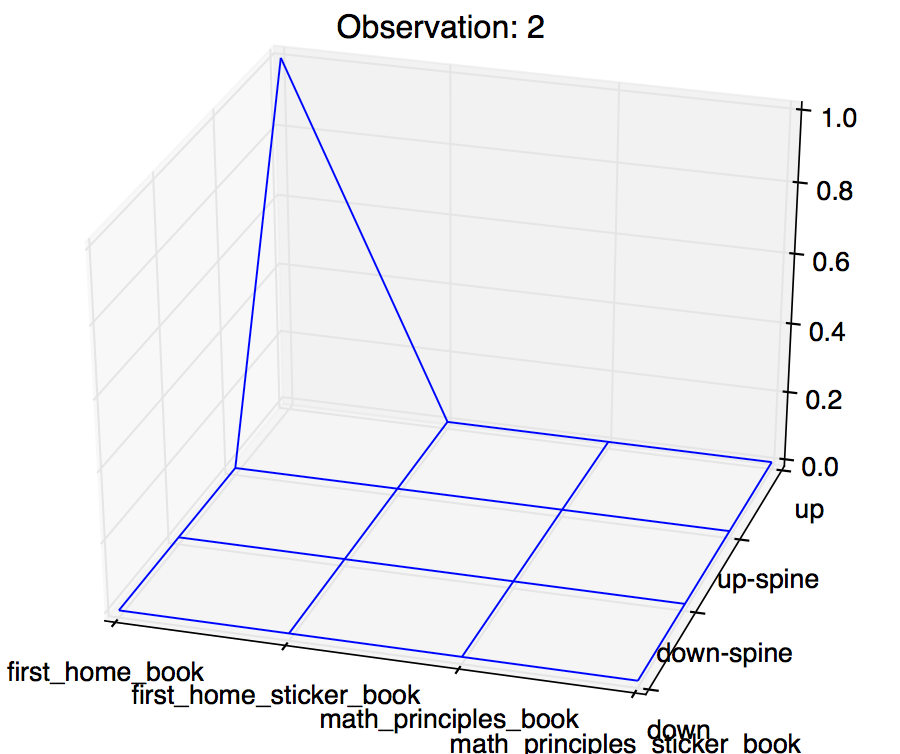
\includegraphics[scale=0.4]{pics/experimentObs2.png}
            \end{tabular}
            \caption{Posterior probabilities of object and pose for the (left) ambigious observation and (right) unambiguous observation.}
            \label{fig:expObsPost}
        \end{figure}

        Of the four actions, staying and rotating result in similarly ambigious poses resulting in an expected entropy of $0.7$. Flipping the book over, with and without rotating, lead to similarly unambigious poses with an expected entropy of $0.0$. Because both actions lead to comparably unambigious poses, the best action can be decided based on some criteria such as minimum energy. After flipping the book, the robot observes the cover of the book (\figref{fig:expObs} left)and knows precisely what book it is observing (\figref{fig:expObsPost} right).

        The expected entropy is calculated again for each action and they are all $0.0$. This may seem peculiar, but recall that the next posterior is simply an update of the previous posterior (\eqref{eq:fullPosterior}, \eqref{eq:fullPosteriorSimplified}, \eqref{eq:posteriorUpdateGeneral}, \eqref{eq:posteriorUpdateComputation}). Once the object recognition algorithm has converged to 100\% certainty, the updated posterior will always remain the same as the previous posterior. Even if the object is moved back into an ambigious pose, the model remembers its previous observations and recalls the correct object. 

    % \subsection{Discussion}
    % discuss being feature agnostic
    % discuss how to cover the other two canonical examples
    % assumptions
        % perfect actions (no noise)
        % discrete poses 
        % we see one object at a time
        % we see a known object
